\documentclass{beamer}

%\usepackage{qtree}
\usepackage{beamerthemetree}
%\usepackage{beamerthemesplit}
\usepackage{color}
\usepackage{lingmacros}
\setbeamertemplate{footline}[frame number]
\usepackage{graphicx}
%\usepackage{xyling}
%\usepackage[swedish]{babel} 
\usepackage[latin1]{inputenc} 
\usepackage{natbib,avm}
\newcommand{\newblock}{}
\usepackage{hyperref}


\title{An Introduction to  Semantics using Type Theory with Records\\
  Lecture 1           }
\author{Jonathan Ginzburg\\
Universit\'e Paris-Diderot, Sorbonne Paris-Cit\'e\\
Robin Cooper\\ 
University of Gothenburg}
\date{}

\AtBeginSection[]
{
   \begin{frame}[plain]
       \frametitle{Outline}
       \tableofcontents[currentsection]
   \end{frame}
}

\newcommand{\backgroundyellow}{\beamertemplateshadingbackground{yellow!40}{magenta!20}}
\newcommand{\backgroundwhite}{\beamertemplateshadingbackground{white!100}{white!100}}
\newcommand{\ba}{\begin{avm}}
\newcommand{\ea}{\end{avm}}


\newenvironment{display}{\begin{center}}{\end{center}}

%
% Reference the next example in the text:
%
\newcommand{\nexteg}[1]{\addtocounter{examplectr}{1}(\arabic{examplectr}{#1})\addtocounter{examplectr}{-1}}
%
% Reference the previous example in the text:
%
\newcommand{\preveg}[1]{(\arabic{examplectr}{#1})}
%
% Reference examples by relative offsets:
%
\newcommand{\egnum}[2]{\addtocounter{examplectr}{#1}(\arabic{examplectr}{#2})\addtocounter{examplectr}{-#1}}
%
%
% ENVIRONMENTS
%
% Examples Environments
%
\newcounter{examplectr}
\newcounter{subexamplectr}[examplectr]
\renewcommand{\thesubexamplectr}{\alph{subexamplectr}}
%
% Sub-example Macro:
%
\newenvironment{subex}%
   {%\vspace*{-.8\baselineskip}
     \begin{list}
       {\alph{subexamplectr}.}%
       {\setlength{\topsep}{0in}
        \setlength{\leftmargin}{1em}%{0.25in}
        %\setlength{\listparindent}{-2em}
        %\setlength{\labelsep}{\baselineskip}
 \usecounter{subexamplectr} }
       }%
   {\end{list}}
%
% Single Example Macro
%
% \newenvironment{ex}%
%    { \refstepcounter{examplectr}
     
% \bigskip

%     % \begin{list}
%       % {
%        (\arabic{examplectr})%}%
%        % {%\setlength{\topsep}{0in}
% %         \setlength{\leftmargin}{4em}%{0.75in}
% %         \setlength{\labelsep}{\baselineskip}
% % }
%         \hspace*{1em}\begin{minipage}[t]{4in} 
% %\item
%    }%
%    {\end{minipage}

% \bigskip

%     %\end{list}
% }
% %
% % End of example macro
% %
\newcommand{\bit}{\begin{itemize}}
\newcommand{\pa}{\pause}
\newcommand{\eit}{\end{itemize}}
\newcommand{\ben}{\begin{enumerate}}
\newcommand{\een}{\end{enumerate}}
\newcommand{\ignore}[1]{}
\newcommand{\eeen}{\eenumsentence}
\newcommand{\subegref}[2]{(\ref{#1}\ref{#2})}

%\newcommand{\beg}{\begin{ex}}
%\newcommand{\eeg}{\end{ex}}
%\newcommand{\bseg}{\begin{subex}}
%\newcommand{\eseg}{\end{subex}}


\newcommand{\egstack}[1]{\begin{tabular}[t]{@{}l@{}} #1 \\ \\
  \end{tabular}}

%Records

\newcommand{\record}[1]{$\left[\mbox{\begin{tabular}{lcl} #1
\end{tabular}}\right]$} 
\newcommand{\smallrecord}[1]{$\left[\mbox{\begin{tabular}{@{}l@{}c@{}l@{}} #1
\end{tabular}}\right]$}

\newcommand{\field}[2]{#1 & = & #2}
\newcommand{\tfield}[2]{#1 & : & #2}
\newcommand{\smalltfield}[2]{#1:#2 & &}
\newcommand{\mfield}[3]{#1=#2 & : & #3}
\newcommand{\smallmfield}[3]{#1=#2:#3 & &}
\newcommand{\hfield}[2]{{\sc #1} & & #2}

\ignore{


The interactive stance to semantics moves to an analysis of semantics
which can characterize the potential for misunderstanding, rejection,
and correction. 

1. basic desiderata.
1.5 sexy stuff we will do and need to do
2. plan of course
(a) eliminate slides 1-16. Keep: 17-25. eliminate: 26-43. keep: 44-61. That's < 30 slides.
If one wanted, one cd also add as a bit of extra data slides 12-15.
If not, the alternative is to add a couple of slides wrapped around slide 22 (the slide titled Pay Off) because we need a slide or three where we  present some of the amazing problems we plan to solve.

}

\begin{document}

\frame[plain]{\titlepage}
%\frame[plain]{\frametitle{Outline}\tableofcontents}

\begin{frame}\frametitle{ Basic information about the course      }





\begin{itemize}
\item[] {\bf Lecturers:} Robin Cooper, Jonathan Ginzburg

%\item[] {\bf Office:}  A06, Charles V

%\item[] {\bf Phone:} 01.57275814, 06.42547226

\item[] {\bf Email:} {\tt cooper@ling.gu.se}, {\tt yonatan.ginzburg@univ-paris-diderot.fr}

\item[] {\bf Office hours:} by appt

\item[] {\bf Website}:  \url{https://sites.google.com/site/semttr}



\end{itemize}

\end{frame}

%\section{Interaction and Grammar}

\begin{frame}\frametitle{     The Primacy of  Spoken Language }

\bit

\item Uncontroversial: Spoken language is the primary form of language, both from the
  point of view of language evolution and language acquisition.

\item Controversial: {\bf interaction is built
  into the grammar.}

\eit
\end{frame}




\begin{frame}\frametitle{ Interaction and Grammar}
\bit
\ignore{\item Few would seriously dispute the importance of studying
conversational interaction. 

\item The dominant paradigms in grammar and semantics have, on the
whole, abstracted away from interaction, viewing it as somebody else's problem.
}
\item Given the state of the art, a simple {\bf actual} conversation such as (\ex{1}), still constitutes a significant
challenge to formal grammar of just about any theoretical
flavour.

\eit
\end{frame}


\begin{frame}\frametitle{3 People trying to print a file
    (ca. 1990)} 

{\tt John:	Okay which one do you think it is?\\
\hspace{1cm}	Try F1 F1  again and we'll get \\
Sarah:	Shift and F1?  \\
Sue:	It's,  no. \\
John:	No, just F1  F1. \\
Sue:	It isn't that. \\
John:	F1. \\
	Right, and that tells us \\
Sue:	It's shift F7.} 

\hspace{1in} (from the British National Corpus)
%\hfill\hyperlink{distance}{\beamergotobutton{Back}}

%\hfill\hyperlink{mult}{\beamergotobutton{Back}}
\end{frame}

\begin{frame}\frametitle{3 People trying to print a file
    (ca. 1990)} 

\bit
\item a rather humdrum conversation from the British
National Corpus (BNC).


  
\eit

\end{frame}

\begin{frame}[label=runningex1]\frametitle{Fragments in conversation: frequency}

\bit
\item Distinguishing characteristic of spoken language---high
  frequency of {\it fragments}
\eit
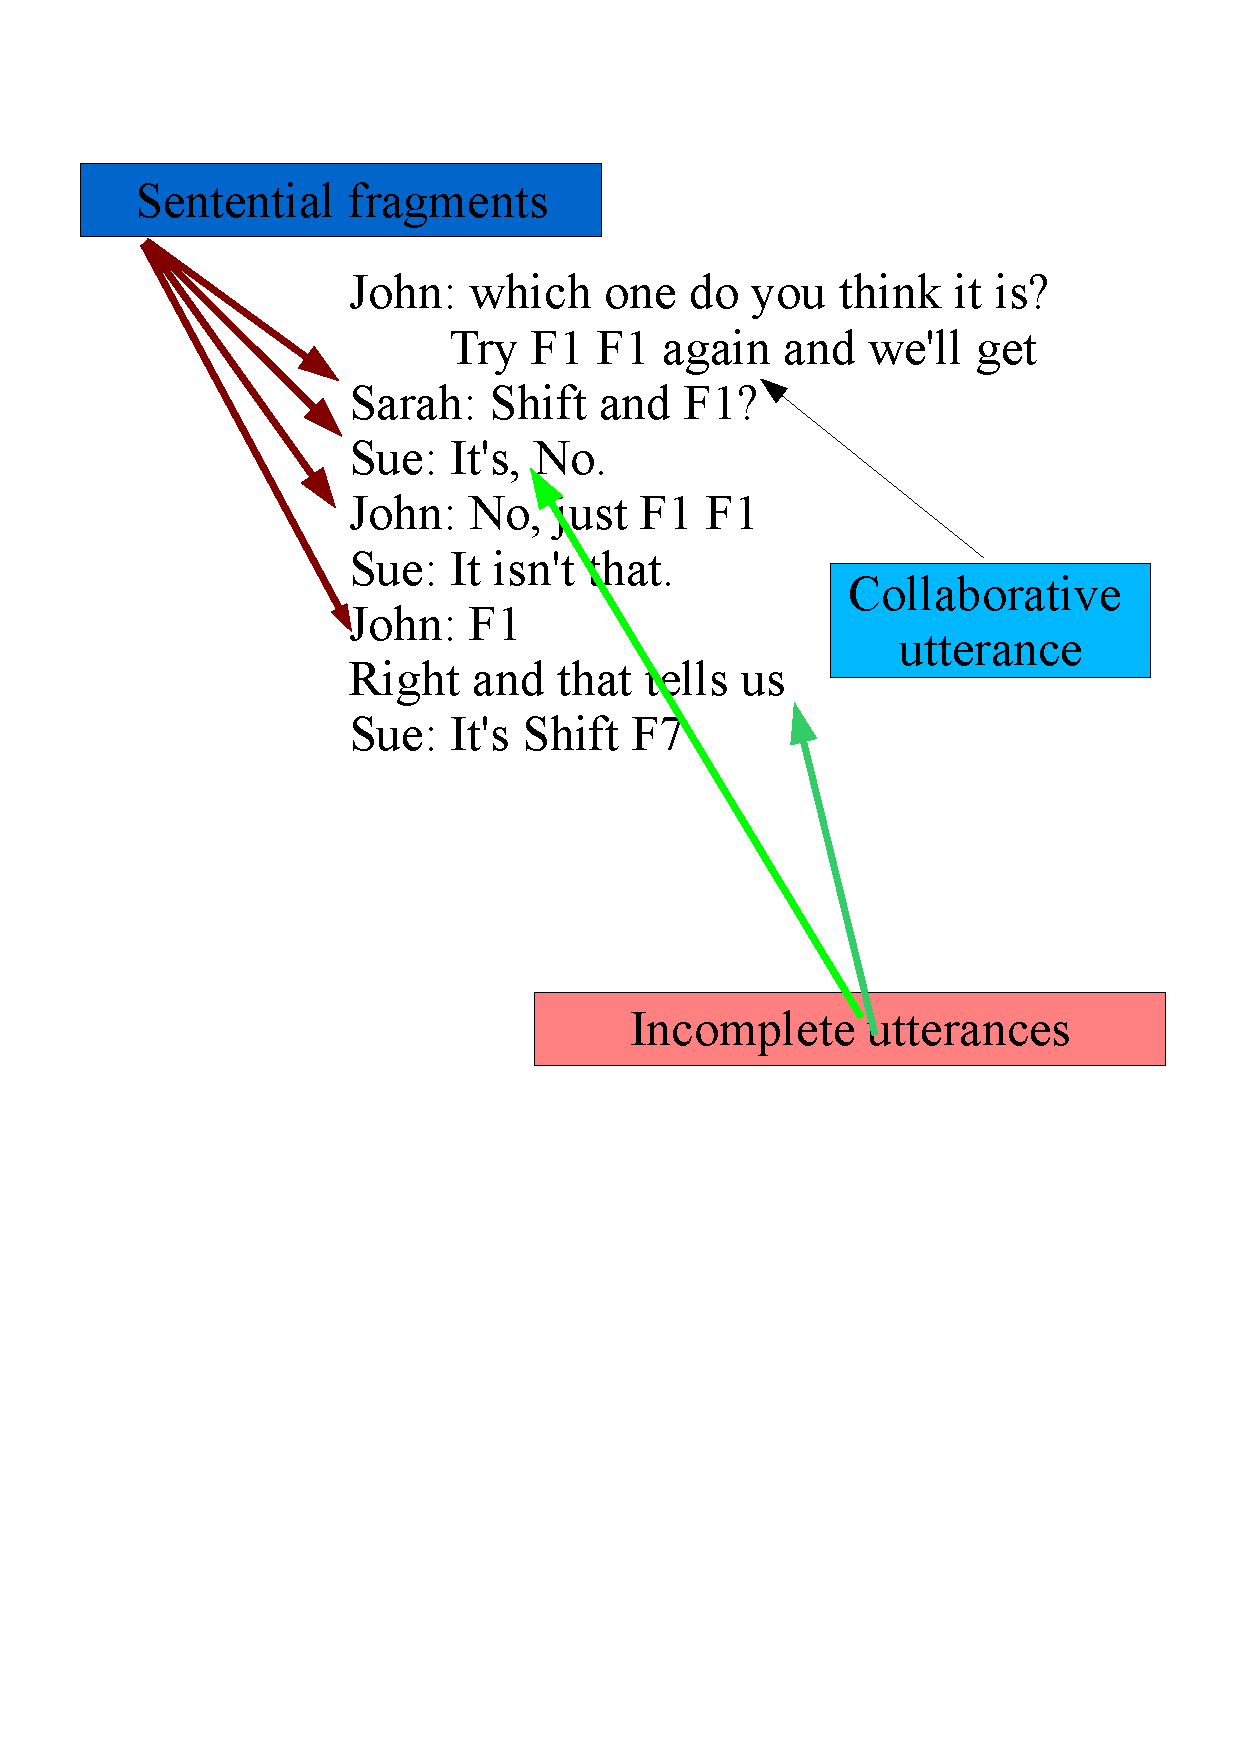
\includegraphics[height=10cm,width=8cm]{challenges0.pdf}

%\hfill\hyperlink{SF1}{\beamergotobutton{Back}}
\end{frame}


\begin{frame}\frametitle{Challenges to semantic/discourse theories}

%\begin{figure*}[!h]
%\begin{center}
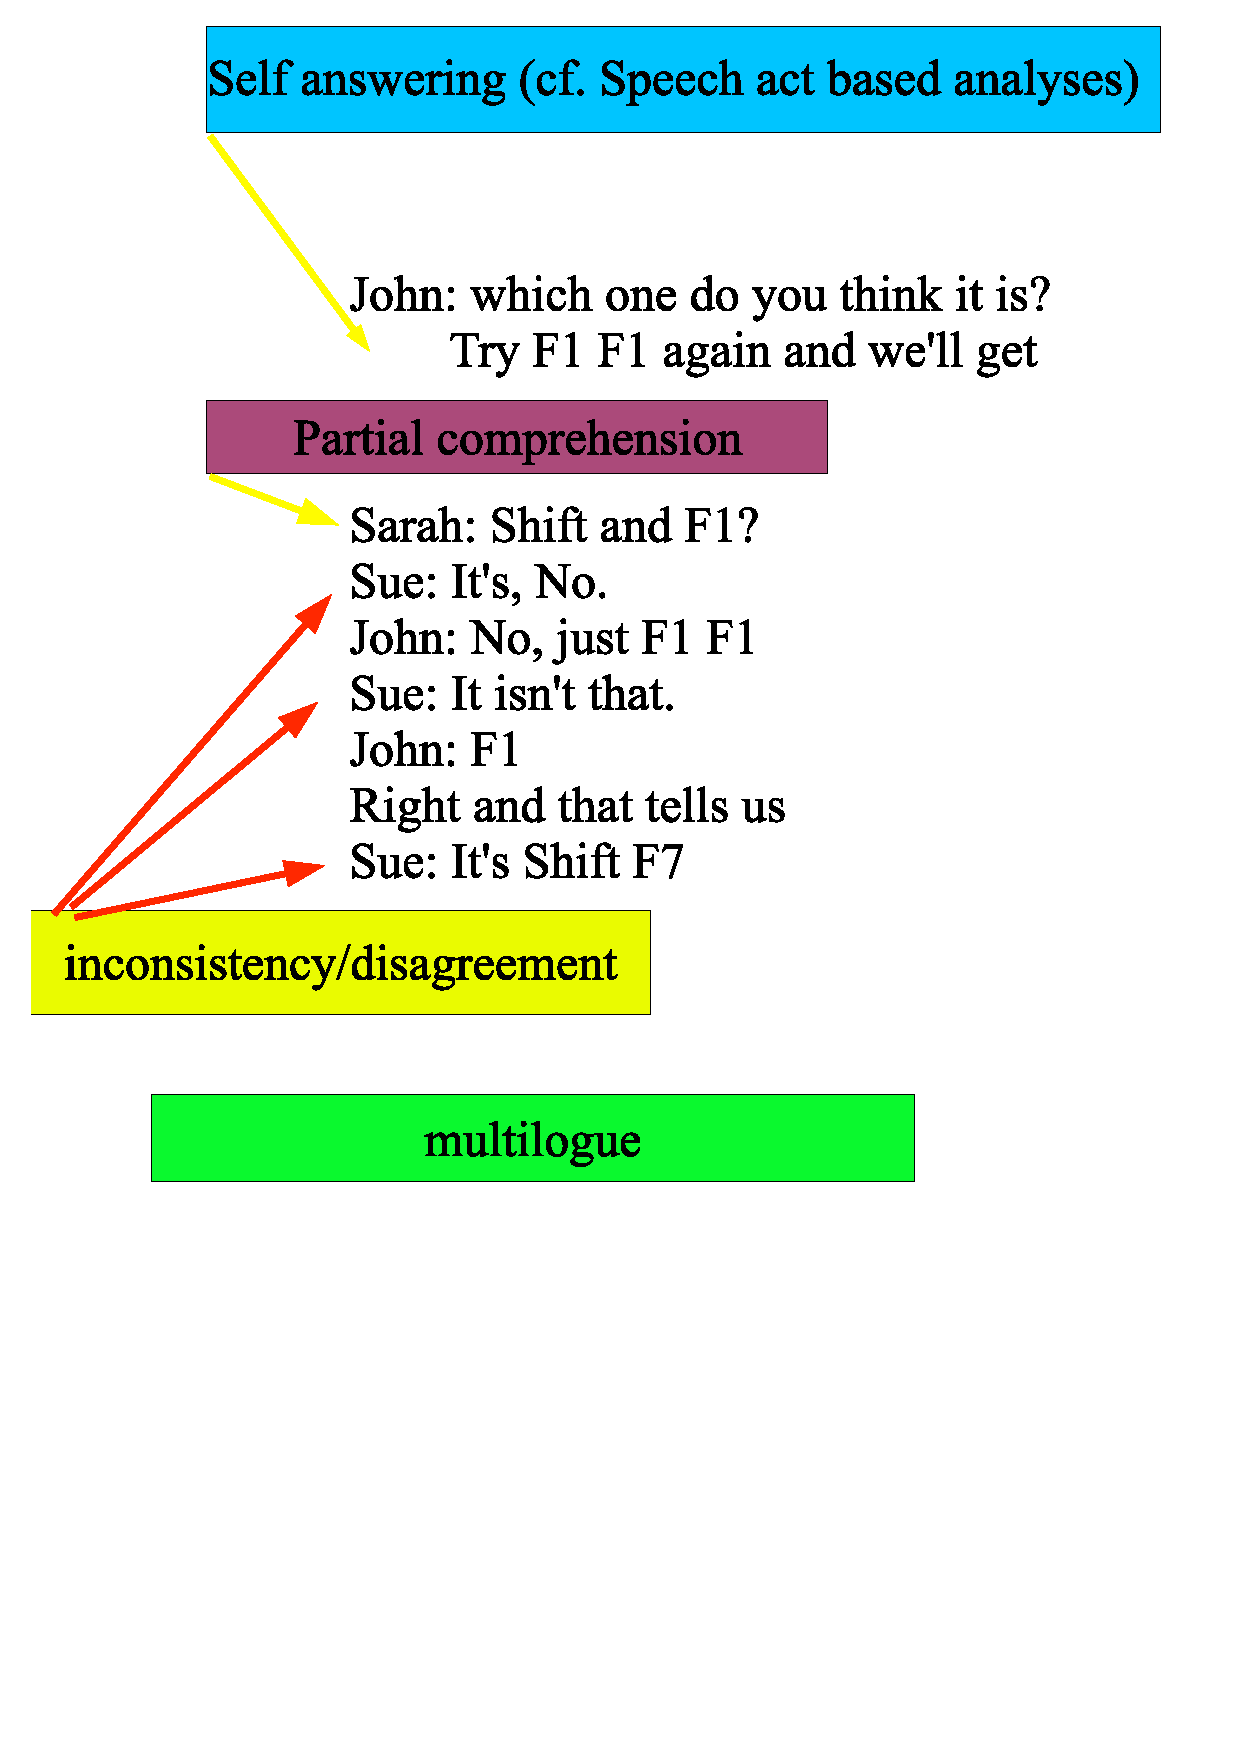
\includegraphics[height=10cm,width=8cm]{challenges1.pdf}
%\caption{Sketch of Interrogatives type hierarchy from Ginzburg and Sag 2000} \label{int-hi}
%\end{center}
%\end{figure*}




\end{frame}

\begin{frame}\frametitle{3 People trying to print a file}

\bit

\item Making sense of all
these phenomena in a systematic way is a challenge undertaken in the
Type Theory with Records (TTR)--based dialogue framework KoS 
KoS
(\cite{ginzburg-iwcs94,larsson-diss,gc-lp02,purver-diss,raquel-diss,ginzburg-buke}). 


\item We will illustrate throughout the course how the
various ingredients that make up TTR allow this challenge to be met.

\item We will revisit the example at the end of the course \ldots

\item But for now the first issue is: 
\eit


\end{frame}

\frame[allowframebreaks]{\frametitle{ Why Type Theory with Records?}

We will motivate the need for the framework with arguments from:

\ben
\item {\bf Semantic ontology}: Why not possible worlds? 

\item {\bf syntax-semantics interface}: Why is a Typed Feature Structure
  (TFS)-based
  syntax-semantics insufficient? 

\item {\bf grammar and interaction}:  meaning in dialogue can only be
expressed with reference to either highly incremental context (e.g.\
Non sentential utterances, dysfluencies) or very global, conversation--genre context. A
framework like TTR is needed to model such grammar--context relations.

\ignore{\item \textbf{language as a system in flux}:  grammar, including
  meaning, is not something that is fixed once and for all.  Our
  language is in a constant state of change as we are influenced by
  interaction with others.  We attempt to capture this by focussing
  our attention on formulating resources which are available to an
  agent and which allow the construction of specific grammars
}
\een


}

\frame[allowframebreaks]{\frametitle{ Why Type Theory with Records: Semantic ontology }

\bit

\item Possible worlds semantics has intrinsic problems, ones Montague
  was aware of  when he first used it in his seminal papers in the
  1970s.

\item Lack of fine grain / logical omniscience: necessarily equivalent
  propositions cannot be distinguished.

\item So the following sentences are predicted to have the same truth
  values:

\eeen{\item Jill believes that Jill is identical to herself.

\item Jill believes that Jill's father is identical to himself.

\item Jill believes that $e^{i\pi} + 1 = 0$
}

\item These problems are often ignored because of the assumption that
  attitude sentences are complex in any case and the difficulties for
  possible worlds semantics can be contained.



\item Regardless of whether one can maintain this view about attitude
  sentences, we present problems for possible worlds in a domain which
  is more difficult to quarantine---negation.

\item In most frameworks sentences like (\ex{1}a,b) are taken to
  denote the same entity:

\eeen{\item Is Gu Xilai guilty?
\item Is Gu Xilai not guilty?
}

\item We will offer extensive linguistic evidence against this
  conclusion. 

\item We will develop
  treatments of negation and questions in TTR that can
  both distinguish between sentences like (\ex{1}a,b), while ensuring that
  sentences like (\ex{2}a,b) remain equivalent:

\eeen{\item Bo saw Jill leave.
\item Bo saw Jill leave and Max enter or Max not enter.
}

\eeen{\item Jill knows whether Gu Xilai is guilty.
\item Jill knows whether Gu Xilai is not guilty.
}
\eit
}

\frame[allowframebreaks]{\frametitle{ Why Type Theory with Records:
    Syntax Semantics interface }

\ignore{
1.  tools used in formal semantics, functions, function application:
important for semantic combination, quantification, questions,
meaning/content/context relation 

2. feature based grammar, feature structures, unification
tfs's: basis for capturing generalizations at various levels of grain in grammar, for characterizing
utterance types, unification: combining partial information

3. meanings as functions can be brittle; unification as semantic glue
can lead to unintuitive results.

4. TTR has operations equivalent to both, allows to synthesize best of both. 




}

\bit

\item Two types of approaches to synsem interface.

\item[1.] $\lambda$-calculus driven (inspired by Montague semantics): 
  function--based.
\bit
\item function application as semantic glue.

\item Generalized quantifiers as functions (from properties to
  propositions)

\item Questions as propositional abstracts.

\item Meanings as functions from contexts to contents.
\eit
\newpage

\item[2.] Feature based grammar: uses typed feature structures and
  unification.
%(e.g.\ HPSG,  CxG, MRS)

\bit

\item basis for capturing generalizations at various levels of grain
  in grammar (lexical hierarchies, constructional hierarchies)

\item allows utterance types (`signs')---parallel representations of
  various grammatical dimensions: important for quotation,
  metacommunicative interaction:

\eeen{\item `Bo' is a noun.
\item `Bo starts with b.
\item `Bo' is used to refer to a person named `Bo'. (\cite{gc-quot12})
}


\item unification: useful for combining partial information, e.g.\ in
  incremental processing

\eit

\item $\lambda$-calculus driven approaches don't have feature
  structures and unification.

\item feature-based grammar approaches don't have functions and
  binding.

\item TTR is both function--driven and has feature structures with
  unification. We will give examples of how the two complement each other as we progress.

\eit
}














\frame[allowframebreaks]{\frametitle{ Why Type Theory with Records:
    grammar and interaction}

\bit
\item Accommodating the fact that spoken language involves interaction
typically viewed as external to the grammar as such.

\item to the extent we accept that indexicals such as `I', `You',
`Here', and `Now' need to be accommodated by the grammar
a similar claim can be made for the NSUs exemplified in (\ex{1}):


\item The meaning of  words or constructions
involves notions that irreducibly involve notions of interaction. 

{\small

\eeen{\label{nsu-in-gram1}
\item Ann: Can you hear the birds singing?	Listen.
James:		Er (pause) {\bf yeah.}
Ann:	Can you hear?
Bryony: I hear birds singing.
Ann:	You can hear the birds singing.
{\bf	Yes.}  %(BNC KB8, 2110--2116)
\item Ann:	Well put it on the draining board and I'll wash it and
  then put it back (pause) James:	Right, I'll see ya tonight
Ann:	{\bf Mhm, mhm} (pause)
James:	Tarrah
Ann:		mm, {\bf bye}   [conversation ends] %(BNC KB6, 7148-7152)


\item  Tim:           Those pink things that af after we had our lunch. 
 Dorothy:           {\bf Pink things?} 
 Tim:          Yeah.           Er those things in that bottle. 
 Dorothy:          Oh  I know what you mean.
          For your throat? 
\item Cherrilyn:          Are you still (pause) erm (pause) going to Bristol 
(pause) on Monday? Fiona:          Dunno.  Cherrilyn:          No?
Fiona:          I dunno.          Doubt it, why? (={\it Why do you 
ask if I'm going to Bristol?})
}}

\newpage
\normalsize
\eeen{
\item A: {\it Yes.}; meaning of `yes': $p$, where $p?$ is the current issue
  under discussion.

\item A:{\it  Bye.}; meaning of `bye': A seeks to disengage from
a  conversation with B which has involved at least some discussion.

\item A: {\it mmh.}; meaning of `mmh': A acknowledges understanding of B's
latest utterance. 

\item B: Did Jo leave? A: {\it Jo?}; {\sf intended content} meaning of
  reprise fragment `u?': A asks B what is the intended reference of  
B's (sub-utterance) u under condition of phonological segmental identity.

\item B: Did Jo leave? A: {\it Why?};  meaning of metacommunicative
   `Why?': A asks B of the cause of an utterance by B, an utterance
  the issue which it raises remains under discussion.
}

\newpage

\item Need formal theory that provides notions such as `current issue
  under discussion', `disengagement from conversation', `
  acknowledgement of understanding', `ask  intended reference of
  other's utterance', \ldots
\item KoS (\cite{ginzburg-iwcs94,larsson-diss,gc-lp02,purver-diss,raquel-diss,ginzburg-buke})
links up: the external world, grammar, and interaction.


\item Fundamental to KoS is the dynamic strategy to meaning, pioneered by
Stalnaker, Lewis ,Kamp, Heim, Barwise, Groenendijk and Stokhof et al---the
meaning of a linguistic form is explicated in terms of the effect its
use has on existing commonly shared contextual ``resources''.  

\item  This suggests 
thinking of context as structured by resources which conversational participants keep 
track of, as demonstrated by linguistic evidence.

\item Working out what these resources are and how to model interaction
in their terms will be a focus of lectures 3 and 4.

\eit
}

\begin{frame}\frametitle{Linking up the external world, grammar, and interaction}

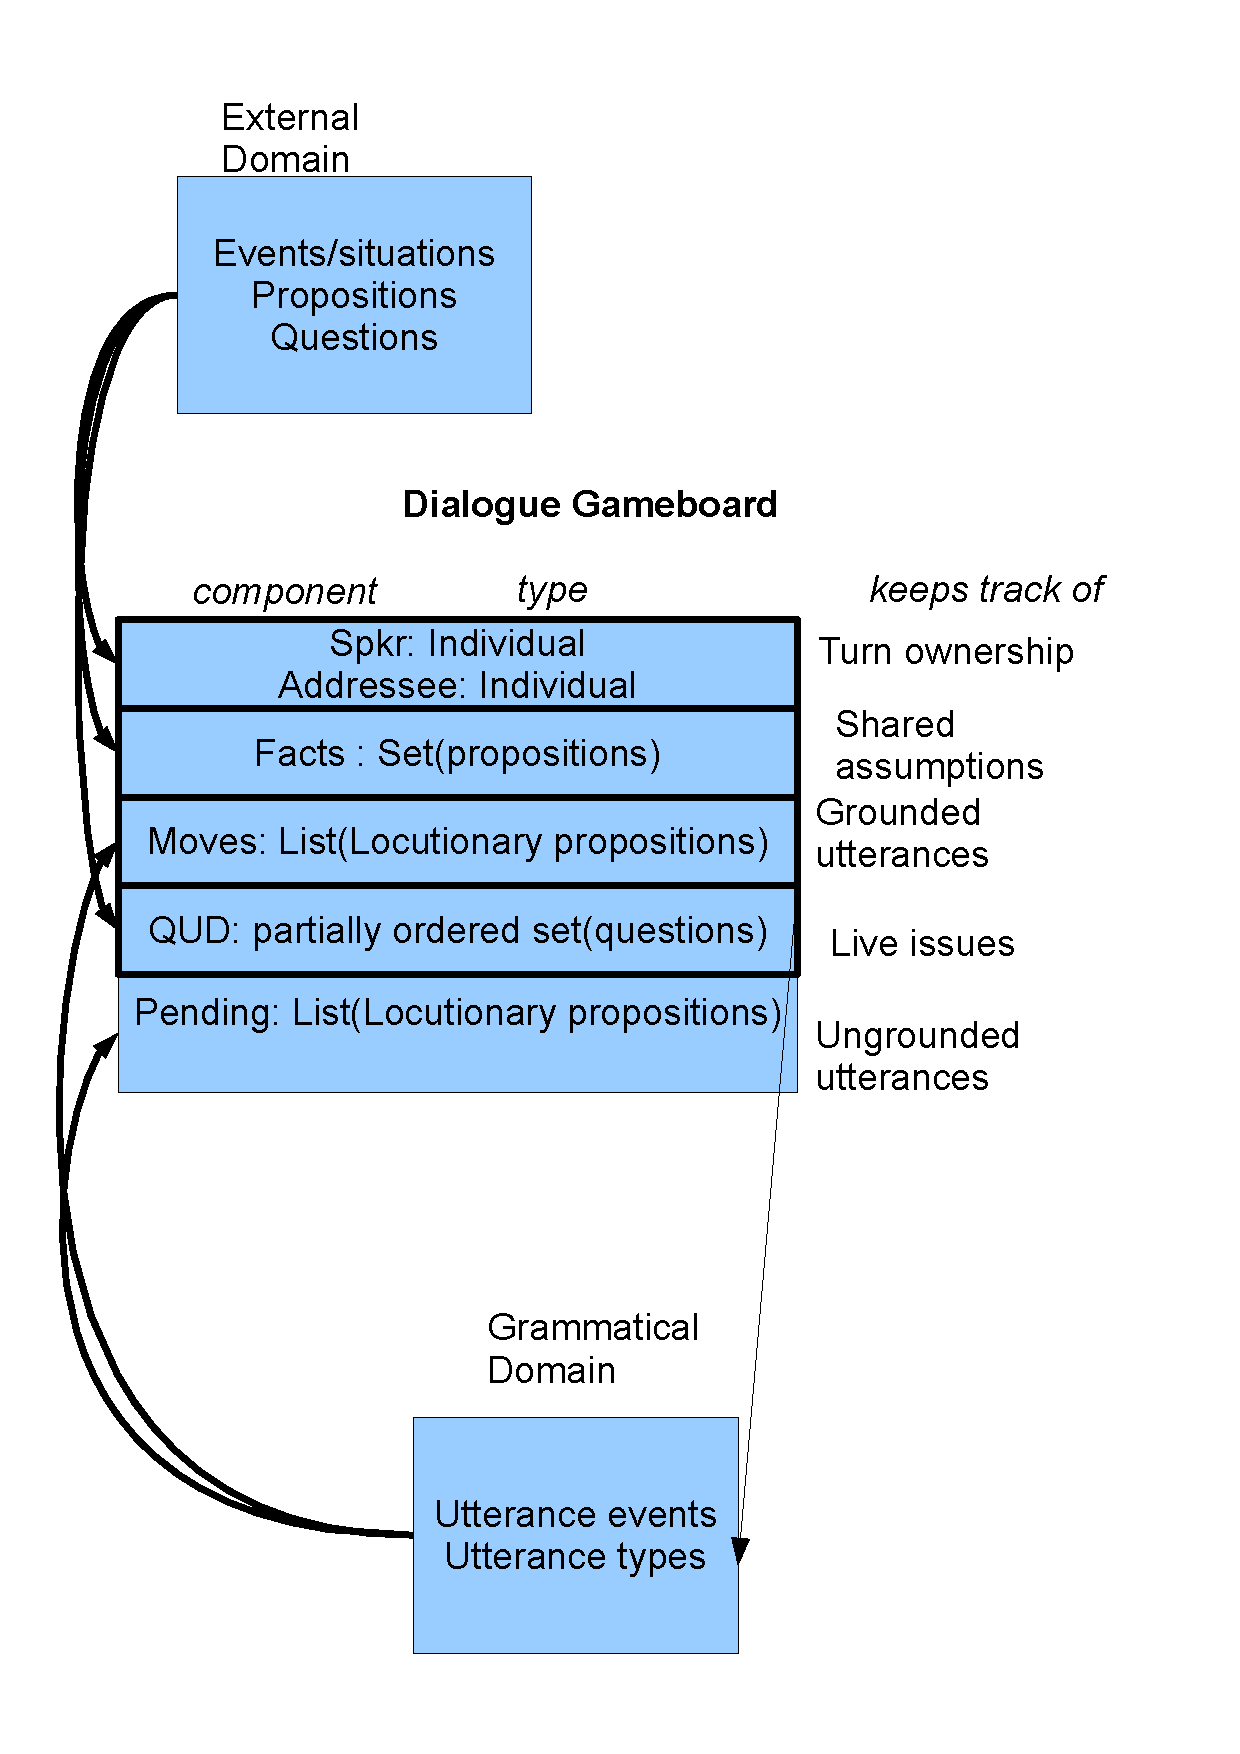
\includegraphics[height=8cm,width=12cm]{sum2.pdf}

\end{frame}
\ignore{
\begin{frame}\frametitle{Type Theory with Records (TTR) }
\bit

\item For this purpose we will use Type Theory with Records (TTR). 

\item TTR is a formalism that allows
us to incorporate insights from Situation Semantics, Montague
Semantics, Discourse Representation Theory,  Head-driven Phrase
Structure Grammar, and Semantic Frame Theory. 

\item We will show how it
can be used to model semantic ontologies, interaction, and to write
dialogically-oriented grammars.


\eit
\end{frame}
}
\ignore{
\begin{frame}\frametitle{Pay Off [delete?]}
\bit

\item \textcolor[rgb]{0.98,0.00,0.00}{Conversation from micro (disfluencies) to macro (conversational genres, multilogue)}
\item \textcolor[rgb]{0.98,0.00,0.00}{Conversation: Opening, middle game, ending }
\item \textcolor[rgb]{0.98,0.00,0.00}{Empirical benchmarks for NSUs and metacommunication from corpus
  studies on the British National Corpus, child language data}
\item New perspective on traditional semantic concerns:
\textcolor[rgb]{0.98,0.00,0.00}{negation},  quantification, anaphora, 
\item \textcolor[rgb]{0.98,0.00,0.00}{Detailed theory of relevance}, which allows us also to talk about Gricean
  {\it irrelevance}.
\eit
\end{frame}
}

\begin{frame}\frametitle{Course Plan}
\bit

\item  {\bf Lecture 1}: Motivation for using TTR; Introduction to TTR

\item {\bf Lecture 2}: Grammar in TTR: frames and lexical semantics;
  

\item {\bf Lecture 3}: A theory of abstract entities (propositions,
  questions, outcomes) and illocutionary
  interaction: analysis in terms of dialogue game boards; Negation.

\item {\bf Lecture 4}: Unifying metacommunicative and illocutionary
  interaction; Generalized quantifiers and clarification.

\item {\bf Lecture 5}: Non-sentential utterances; extensions:
  disfluencies, multilogue, conversational genres.

\eit
\end{frame}

\bibliographystyle{natbib}\bibliography{newest-jg-fin}
\end{document} 

\ignore{\frame[allowframebreaks]\frametitle{Linking up the external world, grammar, and interaction}
\bit



\item By combining the view of context that this leads to with a perspective
originating from Artificial Intelligence  work on the design of
dialogue systems (following e.g.\
  \cite{allen-perrault80})  will enable us to explicate the existence
  of interaction conventions specific to a particular domain or
  genre. 

\item In this way offering formal counterparts akin to Wittgenstein's
  {\it language games} \cite{witt53} and Bakhtin's {\it speech
    genres} \cite{bakhtin1986sga}.
\eit\end{frame}
}




\ignore{
\begin{frame}\frametitle{Course Plan}
\bit
\item


\eit
\end{frame}
}

\ignore{
\begin{frame}\frametitle{ Today      }
\ben

\item Understand basic assumptions of semantic theory needed to
  analyze NSUs
  and the problems they encounter when applied to conversation.
\item TTR: the basics.
\item A theory of events and situations: frames and lexical semantics
\een
\end{frame}
}


\section{Communitarian Semantics bumps into Conversation}


\begin{frame}
\frametitle{From Communitarian Semantics to the Interactive Stance}

\begin{itemize}

\item Semantics as practised highly productively since Frege:
\begin{itemize} \item characterizing {\it successful communication}:
\bit
\item {\it the proposition expressed by a sentence in context}
\item {\it the referent of an NP}
\item {\it anaphoric/presuppositional potential}
\eit
\item abstracting away from individual differences, from the
{\it communicative process}
\end{itemize}
\item {\it Communitarian Semantics}
\end{itemize}

\end{frame}

\begin{frame}
\frametitle{From Communitarian Semantics to the Interactive Stance}

\bit

\ignore{\item We have already seen data that requires one
  to interleave the communicative process into the semantics---the
  NSUs in (\ref{nsu-in-gram1}). 
}

\item A variety of data  we will see today will lead us to propose an
  alternative, more general perspective to our semantic
  enterprise---the {\sf interactive stance}. 

\item The {\sf interactive
    stance} involves taking seriously the fact that communication
  involves multiple agents with distinct beliefs and desires and
  places importance on explicating the potential for misunderstanding,
  rejection, and correction, as well as success.

\eit
\end{frame}
\ignore{
\begin{frame}
\frametitle{From Communitarian Semantics to the Interactive Stance}

\begin{itemize}

\item
  Adopting the {\sf interactive stance} will allow us to incorporate
  into  formal semantic theory insights from two important bodies of work.

\item  Conversation Analysis (e.g.\ \cite{sjs77,schegloff87}), which lead
  the way in recognizing the fundamental importance of {\it repair}, and
 
\item  Clarkian psycholinguistics (e.g.\ \cite{clark96}), which has offered
  detailed documentation of {\it grounding}---the process by means of
  which content becomes part of the common ground.

\item The (or um a) basic requirement
on semantic theory:

 \textcolor[rgb]{0.98,0.00,0.00}{The
  ability to characterize for any utterance type the update that
  emerges in the aftermath of successful grounding and the full range
  of possible Clarification Requests otherwise}.


\end{itemize}

\end{frame}


}





\begin{frame}
\frametitle{Communitarian Semantics: some
    assumptions }

\ignore{
\begin{itemize}

\item {\sf Contextualized Lewisian Regularity}: whenever A utters $S$ 
with meaning $\mu$ in $c$, A communicates that P, where P = $\mu[f]$, 
$f$ is the assignment $c$ provides for $\mu$, and B acquires the 
belief that P. 

\item {\sf Equal Access to Context:}  As a
conversation proceeds a common ground emerges: A has her turn, reaches
a transition relevance point (TRP); Then either A proceeds or B takes
over {\bf from the common ground point at which A spoke.}


\item {\sf The supra-contextual nature of Semantics}: Semantics 
associates meanings with sentences and constituents of sentences.

\end{itemize}
}

\end{frame}

\begin{frame}
\frametitle{ Meaning v.\  Content}

\begin{itemize}
\item {\bf Meaning v.\ Content} (Montague, Kaplan, Bar Hillel, Cresswell, Barwise and Perry):
\begin{itemize} \item {\em
  character/meaning},  associated with sentences or types of
utterances, 

\item {\it content/interpretation},  associated with sentences--in--context or utterances.
\end{itemize}
\pause
\item   The basic task of a
semantic analysis--- specify the meanings associated
with expressions (platonic entities, unlocated in
space or time).  
\ignore{\item A meaning of an expression $E$--- a rule which allows a conversationalist to
calculate, given a context $c$, what content is associated with $E$ in
$c$.  
}
\pause
\item Alternative construal:  a meaning---associated with an utterance type, where an utterance is a
spatio-temporally located event involving the sequential enunciation
of one or more words.
\pause
\item This perspective proffered originally in
\cite{bp83,gp90,cp94,poesio98}), but has generally aroused scant interest.

\end{itemize}
\end{frame}

\begin{frame}
\frametitle{ Meaning v.\  Content}

\begin{itemize}


\item {\it The supra-contextual nature of Semantics}: Semantics 
associates meanings with expressions.



\item This notion of a meaning as a contextual use rule can be formalized as 
a function from {\it contexts} to {\it contents}.    
(\ref{meaning-ex1}) is a simple example of a meaning construed 
as a function:

\eeen{\label{meaning-ex1}
\item I hear you.
\item f: c $\mapsto$ Hear(s,a,t), where s is the speaker in c, a is 
the addressee and t overlaps with the time of c.
}

\end{itemize}

\end{frame}
\begin{frame}
\frametitle{Equal Access to Context }

\begin{itemize}


\item {\it Equal Access to Context:} As a conversation proceeds 
a shared context (the {\it common ground}) emerges: A has her turn, 
reaches a transition relevance point (TRP); Then either A 
proceeds or B takes over {\it from the common ground point at which A 
spoke.}.

\item (\ref{cg1}) exemplifies why {\sf Equal Access} seems a plausible 
assumption: A makes an initial utterance, a query, which either A or B 
can follow up on:

\eeen{\label{cg1}
\item A(1): Who should we invite to the conference?
\item A(2): Perhaps Noam, huh?
\item B(2): Perhaps Noam, huh?}




\end{itemize}

\end{frame}

\begin{frame}
\frametitle{ Lewisian Regularities}

\begin{itemize}


\item Simplifying somewhat,  Lewis (1968) proposes that
a regularity as described below is what underlies the
communicative process involved in conveying `literal import':

\eeen{
\item[] Original Lewisian regularity: 
 Whenever S is uttered, the utterer intends to communicate P and the
hearer acquires the belief P.
}

\item  Now
(\ex{0}) won't work for sentences whose (literal) import
varies with context, the lion's share of actually used sentences. 

\item So replace it with:


\eeen{\item[] Contextualized  Lewisian regularity: Whenever A utters $S$ with meaning $\mu$ in a 
context $c$, A communicates that P, where P = $\mu[f]$, $f$ is the 
assignment $c$ provides for $\mu$, and B acquires the belief that P. }



\end{itemize}

\end{frame}



\begin{frame}
\frametitle{Communitarian Semantics: some
    assumptions }

\begin{itemize}
\item Montague: {\it I fail
to see any great interest in syntax except as a preliminary to
semantics.}  

\item Generally true of formal accounts of context
change (e.g.\ those formulated in Discourse Representation Theory
(\cite{kampreyle93}, in Dynamic Predicate Logic and its relatives
(e.g.\ \cite{gs91,dekker-rlc} and in Segmented Discourse
Representation Theory (\cite{al03}))), with the
important exception of Poesio and Traum's PTT:

\item {\sf Weak Montogovianism}: only the {\it content} of 
utterances ({\it not} their syntactic or phonological properties)
contributes information that persists in the context. 



\end{itemize}
\end{frame}

\begin{frame}[label=Samex]
\frametitle{Motivation for  the Interactive Stance}

%FIX as diagram
 
{\footnotesize
Terry:             Yeah I but think he gave me all his drink. \\
 Damion:             \textcolor[rgb]{0.98,0.00,0.00}{Who?} \\
 Terry:             \textcolor[rgb]{0.00,0.00,0.98}{Sam.} \\
 Damion:             He gave it to you? \\
 Terry:             \textcolor[rgb]{0.00,0.00,0.98}{No, no}, I was (laughing) drinking all his drinks.\\
 Damion:             \textcolor[rgb]{0.98,0.00,0.00}{Which Sam?} \\
 Terry:             Sam, Sam, the one \\
 Damion:             The one \\
 Terry:             who was totally pissed. \\
 Damion:              \textcolor[rgb]{0.98,0.00,0.00}{Oh Fleckerstein or the other one?} \\
 Terry:             No have you got, don't you know the other one? \\
 Damion:              No there's two we know. \\
 Terry:             \textcolor[rgb]{0.00,0.00,0.98}{Yeah.} \\
 Damion:             \textcolor[rgb]{0.00,0.00,0.98}{The one with Kevin} \\
 Terry:              The one with the longish \\
 Damion:             or the other one. \\
 Terry:             it's the other one. \\
 Damion:             \textcolor[rgb]{0.00,0.00,0.98}{Oh right.} (BNC, KR2)
}

\hfill\hyperlink{eqa}{\beamergotobutton{Back}}
\end{frame}

\begin{frame}[label=eqa]
\frametitle{Communitarian Semantics: some
    problematic assumptions}

\begin{itemize}

\item (*) despite being a perfectly normal and unremarkable
conversation points to some very significant issues.

\item Damion spends just about the entire
conversation without a unique referent associated with `he', and `Sam'.

\item Hard to square with
the {\sf Contextualized Lewisian Regularity}: where a function gets
fed its value (a contextual tuple of some kind), yielding a content as
value, or no value whatever if something goes wrong.

\end{itemize}

\end{frame}



\begin{frame}
\frametitle{Communitarian Semantics: some
    problematic assumptions}

\begin{itemize}

\item This technical
quibble is a symptom of a far deeper malaise: with some notable
exceptions to be discussed below, linguistic semantics still operates
under the assumption that {\bf perfect communication}
obtains---nothing does go wrong and interpretation leads to an
identical update on Damian's and Terry's information states. 

\item involves giving up on trying to make sense of conversations such as
the above and most concretely the analysis of the meaning of NSUs there
such as `Who?', `Which Sam', and `Oh Fleckerstein or the other
one?') that express metacommunicative queries.

\end{itemize}

\end{frame}
\begin{frame}
\frametitle{Communitarian Semantics: some
  problematic  assumptions }

\begin{itemize}


\item  The data in (\ex{1}) and
(\ex{2}), involving the resolution of NSUs, are incompatible with (the
above version of) {\sf Equal Access}. 

\item (\ex{1}) illustrates that the
contextual possibilities for resolving the fragment `Bo?' are distinct
for the speaker and the addressee:

\eeen{\label{ttp10}
\item A: Who does Bo admire? B: Bo? \\
Reading 1 (\textbf{ short answer}): Does Bo admire Bo?\\
Reading 2 (\textbf{clausal confirmation}): Are you
asking who BO (of all people) admires?;  \\
Reading 2 (\textbf{intended content }): Who do
you mean `Bo'?
\item  A: Who does Bo admire?  Bo? \\
Reading 1 (\textbf{ short answer}): Does Bo admire Bo?\\
Reading 2 (\textbf{self correction} Did I say `Bo'?)
}
\end{itemize}

\end{frame}
\begin{frame}
\frametitle{Communitarian Semantics: some
  problematic  assumptions }

\begin{itemize}


\item Fragments of this kind, henceforth {\it reprise fragments} (RFs) are
frequent: the \textbf{clausal confirmation}) and \textbf{intended
  content } readings constituting approximately 30\% of all
clarification requests in the British National Corpus.




\end{itemize}

\end{frame}
\begin{frame}
\frametitle{Communitarian Semantics: some
  problematic  assumptions }

\begin{itemize}


\item (\ex{1}) is an even more striking illustration of the phenomenon we
have dubbed the Turn Taking Puzzle (TTP) (see
\cite{ginzburg-ac97}): here the resolution accorded to the bare
`Why?' changes according to who keeps or takes over the turn. 

\item (\ex{1}c) shows that these facts cannot be reduced to coherence or
plausibility---the resolution unavailable to A in (\ex{1}a) yields a
coherent follow up to A's initial query if it is expressed by means of
a non-elliptical form:



\eeen{
\item A: Which members of this audience own a parakeet?  Why?  (= Why own a 
parakeet?)  
\item A: Which members of this audience own a parakeet?  B: Why?  (= Why are you
asking which members of this audience own a parakeet?) 
\item A: Which members of this audience own a parakeet?  
Why am I asking this question?
}

\end{itemize}

\end{frame}
\begin{frame}
\frametitle{Communitarian Semantics: some
  problematic  assumptions }

\begin{itemize}


\item The Turn Taking Puzzle vitiates {\sf Equal Access}, since it demonstrates in a rather
direct way that, at least some of the time, the contextual options
available to one participant are distinct from those available to the
other(s) participant(s).  




\item At the same time, the TTP is not an argument
for solipsism, for instance of a type advocated in Relevance Theory
(\cite{sperber-wilson86}), the only influential approach which
explicitly  avoids assuming {\sf Equal Access}. 

%(Though recent change in SDRT, see FIX).

\item  The TTP
reflects an asymmetry of production, not understanding: it seems clear
that both participants would understand the potential contributions of
the other. 



\end{itemize}

\end{frame}
\begin{frame}
\frametitle{Utterances v. Sentences--in--context }

\begin{itemize}


\item The data in (\ref{utt1}) illustrates that if A makes the 
utterance in (\ref{utt1}(1)) a variety of facts about the utterance 
(in bold face in (2b-e)) potentially enter into the common ground. 


\item  (\ref{utt1}) 
exemplifies two classes of facts about the utterance that become 
presupposable, facts about the content of sub-utterances 
(\ref{utt1}(2b-d)) and also facts that concern solely the phonology 
and word order of the utterance. 


\eeen{\label{utt1} \item[]           

\noindent A(1): Did Mark send you a love letter?\\
B(2b): No, though it's interesting {\bf that you refer to Mark/my
brother/our friend}  \\     
B(2d): No, though it's interesting {\bf that you ask about Mark's epistolary
habits}\\ 
B(2e): No, though it's interesting {\bf that the final two words you 
just uttered start with `l'}
  }

\end{itemize}

\end{frame}



\ignore{
\begin{frame}
\frametitle{ Utterances v. Sentences--in--context}

\begin{itemize}


\item The fact that non-semantic information such as phonology or word order
associated with an utterance needs to filter into the context and stay
there for a while $\not\rightarrow$  all equally {\it
  accessible}.

\item The lion's share of these facts cannot actually be
picked up in fact ellipsis/anaphora.  




 B(3a): (No, though) why? (= {\em why are you asking whether Mark sent me a
love letter}; cannot mean: {\em why do you refer to Mark/my brother/our
friend}, {\em why do you  bring up the sending of love letters} etc)

B(3b): (No, though) Don't you think that's a bit over inquisitive?
(`that' = {\em your asking me whether Mark sent me a love letter})


\item  facts that are easily accessible---{\it
  topical}. Hopefully get to this at the end of the course.

\item  A further
argument for this utterance-based perspective is that the
sub-utterance tokens figure in the content of CRs, as I will discuss
later on.
 

\end{itemize}

\end{frame}
}

\begin{frame}
\frametitle{Weak
  Montogovianism }

\begin{itemize}


\item We have already seen some data that goes against {\sf Weak
  Montogovianism}: the presuppositions about phonology and word order
that emerge in the aftermath of an utterance.

\item  An additional set of
phenomena are phonological and syntactic parallelism phenomena in CRs
and NSUs. 
\item Clausal Confirmation readings require
partial syntactic parallelism: an XP used to clarify an antecedent
sub-utterance $u_1$ must match $u_1$ categorially:



\eenumsentence{\label{para-ex11}
\item A: I phoned him. B: him? / {\#}he?
\item A: Did he phone you? B: he? / {\#}him?
\item A: Did he adore the book. B: adore? / {\#}adored? 
\item A: Were you cycling yesterday? B: Cycling?/biking?/{\#}biked?
}

\end{itemize}

\end{frame}
\begin{frame}
\frametitle{Weak
  Montogovianism }

\begin{itemize}


\item The repetition reading of a RF involve (segmental) phonological 
identity with their source follows from their very nature (`Did you
say \ldots'). And this requirement also applies to
intended content  RFs: 

\eenumsentence{
\item[(i)] A: Did Bo leave? B: Max? (cannot mean: 
intended content reading: {\bf Who are you referring to?} or {\bf Who do you mean?})

 }


\item The persistence of non-semantic information in context is
 very much an empirical question, but discarding {\sf Weak
   Motogovianism} seems a necessary first step in accounting for a
 growing body of work in psycholinguistics that demonstrates the
 existence of non-semantically-based priming (see
 e.g.\ \cite{branigan00,garrodpickering04}).




\end{itemize}

\end{frame}
\ignore{
\begin{frame}
\frametitle{Integrating Semantics and MetaCommunication }

\begin{itemize}


\item Just seen data that calls into question
certain fundamental assumptions of a large body of semantic theory, in
linguistics, the philosophy of language, and computational work, a
view we have dubbed {\sf Communitarian Semantics}.

\item What are the positive
conclusions we can draw on the basis of this data, the nucleus of the
{\sf interactive stance}?

\end{itemize}

\end{frame}
}

\begin{frame}
\frametitle{Integrating Semantics and MetaCommunication }

\begin{itemize}

 \item {\bf  Meaning, Content {\it and} CRification potential}: 
knowledge of meaning includes knowledge of CRification possibilities.
In other words, an important benchmark for any
  semantic theory of dialogue is to accommodate as coherent and
 characterize the range of clarificatory   potential of utterances by
 an interlocutor.


\item {\bf Semantic non-determinism}: the contexts available to
  the conversationalists in the aftermath of an utterance are NOT
  identical, as illustrated by various turn taking puzzles. This
  entails a cognitive architecture in which there is no single common
  ground, but distinct yet coupled Dialogue GameBoards, one per conversationalist.

\end{itemize}

\end{frame}

\begin{frame}
\frametitle{Integrating Semantics and MetaCommunication }

\begin{itemize}

\item {\bf Fine-grained utterance representation}: information
  pertaining to syntactic and phonological aspects of an utterance
not merely the utterance's illocutionary
  {\it content}---on whatever theoretical explication of this
  concept---becomes  presupposed following a grounded
  utterance; This point has also been argued for extensively
    by Massimo Poesio, see
    e.g.\ \cite{potr97,poesio-rieser09}.
\item Also needed for an account of quotation (\cite{gc-quot12})..

\item  This requires a
means of keeping track of the sign information associated with an utterance
  in context after its successful processing. In turn, this necessitates a
  grammatical ontology that furnishes all this information in
  parallel---a {\it sign-based grammar} of some kind 


\end{itemize}

\end{frame}

\ignore{
\begin{frame}
\frametitle{ Integrating Semantics and MetaCommunication}

\begin{itemize}


\item Such phenomena have been studied extensively by
psycholinguists and conversational analysts in terms of notions such
as {\it grounding} and {\it feedback} (in the sense of \cite{clark96}
and \cite{allwood-activity}, respectively.) and of {\it repair} (in
the sense of \cite{schegloff87}).

\item  The main claim that originates with
\cite{cs93} is that any dialogue move $m_{1}$ made by A must be
grounded (viz acknowledged as understood) by the other CP B before it
enters the common ground; failing this clarification interaction
(henceforth {\it CRification}) must ensue. 

\end{itemize}

\end{frame}

\begin{frame}
\frametitle{Integrating Semantics and MetaCommunication }

\begin{itemize}

\item This assumption about
grounding is somewhat too strong, as \cite{allwood-activity} argues.

\item One sided communicative acts are possible, citing examples
such as (\ex{1}). 

\eeen{
\item I was referring to Bertrand Russell but she did not hear
  me. (Example (11) in \cite{allwood-activity}.) 
\item I warned him but he did not hear me. (Example (7) in \cite{allwood-activity}.) 
}

\item  A weakened version provides a
starting point---basic  need to interleave the potential for
grounding/CRification incrementally; the size of the increments being
an important empirical issue. 

\item  From a semantic theory, we might expect
the ability to generate concrete predictions about forms/meanings of
MCI utterances in context. 
\end{itemize}

\end{frame}
}
\begin{frame}
\frametitle{From Truth Conditions to Interaction Conditions }

\begin{itemize}
\item The (or um a) basic requirement
on semantic theory:


 \textcolor[rgb]{0.98,0.00,0.00}{The
  ability to characterize for any utterance type the update that
  emerges in the aftermath of successful grounding and the full range
  of possible Clarification Requests otherwise}.


\end{itemize}

\end{frame}




\bibliographystyle{natbib}\bibliography{newest-jg-fin}
\end{document} 

\section{Communitarian Semantics for conversation: a sketch}


\begin{frame}
\frametitle{ The Semantics of  `yes'}

\begin{itemize}
\item The main difficulty in providing a formal description of `yes' is pinning down 
its contextual background.

\item Informal picture: when `yes' stands alone, it typically serves to affirm a proposition, 
one that has either been asserted or queried:

\eeen{\label{yes0}\item A: Did Suleyman the Magnificent
build the walls of Jerusalem? B: Yes.

\item A: Bo is finally leaving us tomorrow. B: Yes. It's a relief.

\item Robert(1):  It's quite  well established then, your   $\ldots$  uh
  $\ldots$ affair?  Emma(2): Yes.

\item Our affair is quite well established.  
  }

\item In (\ref{yes0}c(2)) Emma conveys to Robert (\ref{yes0}d). How does this come 
about?

\end{itemize}

\end{frame}

\begin{frame}
\frametitle{ The Semantics of  `yes'}

\begin{itemize}
\item The most obvious formal semantics account one 
could offer involves the following three components:

\ben

\item {\bf Meaning:} Emma and Robert know the {\it meaning} of `yes',  
which can be described tentatively as: {\it the proposition currently 
most salient in the context}.

\item {\bf Context:} Emma and Robert are jointly aware of the evolving 
context. In particular, they are both aware that as a result of 
Robert's query the truth or otherwise of {\em the affair is well established} 
became most salient in the context.

\item {\bf Content:} putting 1. and 2. together the content of Emma's 
utterance of `yes' emerges.
\een
\end{itemize}

\end{frame}




\begin{frame}
\frametitle{ Context: basic issues}

\begin{itemize}


\item Having spelled out some basic principles linking meaning, context, and 
content, there are two crucial inter-related issues we need to address
before we can actually spell out the meaning of `yes'. Simply put the 
issues are: 

\ben
\item How is context structured?

\item  How does context evolve?
\een


\end{itemize}

\end{frame}
\begin{frame}
\frametitle{ Contexts in KoS}

\begin{itemize}


\item The answer I will assume for these questions theory derives from work
in KoS

\item  Other
comprehensive accounts of a theory of context for dialogue include
work in the PTT framework (e.g.\
\cite{PoesioTraum97_Conversational,potr98,EDIS,poesio-rieser09}) and
work within Segmented Discourse Representation Theory (SDRT) (e.g.\
\cite{al03,al08}).

 

\end{itemize}

\end{frame}
\begin{frame}
\frametitle{Contexts in KoS }

\begin{itemize}


\item in KoS, there is actually no single context, for
reasons that will soon emerge.

\item Instead of a single
context, analysis is formulated at a level of information states, one
per conversational participant. 

\item What the typed entities depicted in
  (\ex{1}),(\ex{2}) amount to is explained  in the next few lectures.

\item The type of information states
is given in (\ex{1}):

\eeen{\item[] TotalInformationState (TIS):

\ba
\[dialoguegameboard : DGB\\
private : Private
\]\ea
}


 

\end{itemize}

\end{frame}
\begin{frame}
\frametitle{Contexts in KoS }

\begin{itemize}

\item The dialogue gameboard (DGB) represents information
that arises from publicized interactions and, for now, we can identify
it as the public context. 

\eeen{\item[]   DGB (initial definition)

                 \begin{avm}\[spkr: Ind\\
                             addr: Ind\\
                           c-utt : addressing(spkr,addr)\\
                        Facts : Set(Prop)\\
                           Moves : list(IllocProp)\\
                           QUD : poset(Question)\]\end{avm}

}



\end{itemize}

\end{frame}

\begin{frame}
\frametitle{The Dialogue GameBoard }

\begin{itemize}

\item The spkr/hearer roles serve to keep track of turn ownership.

\item {\bf FACTS} represents the shared knowledge conversationalists utilize during a
  conversation. More operationally, information  a
  conversationalist can use embedded under presuppositional operators.

\item {\bf MOVES}:  useful to single out LatestMove,
  a distinguished fact that characterizes  the most
  recent move made. 

\item The main motivation---to segregate from the
  entire repository of presuppositions  information on the basis of which
  coherent reactions could be computed.

\item  Later on see that keeping track of more than just
  the latest move can be useful.

\end{itemize}

\end{frame}

\begin{frame}
\frametitle{The Dialogue GameBoard }

\begin{itemize}
\item {\bf QUD}: (mnemonic for Questions Under Discussion)---questions that constitute a ``live issue''. That is,
  questions that have been {\em introduced for discussion} at a given
  point in the conversation and not yet been {\em downdated}. 

\item There are additional,
  indirect ways for questions to get added into QUD, the most
  prominent of which is during metacommunicative interaction.

\item   Being maximal in QUD ({\sc max-qud})
  corresponds to being the current `discourse topic' and is a key
  component in the theory.




\end{itemize}

\end{frame}
\begin{frame}
\frametitle{ The meaning of `yes'}

\begin{itemize}


\item We can 
hypothesize the following as the meaning of `yes':

\eeen{\label{yes2}
\item[]  {\it The proposition introduced by {\sc latest-move}
into the context}.
}

\item A cursory examination of any conversational corpus will attest that 
this description covers a high percentage of the occurrences of `yes'. 
 
\item Nonetheless, the description is intrinsically incomplete.

\end{itemize}

\end{frame}
\begin{frame}
\frametitle{ The meaning of `yes'}





\eenumsentence{\label{no-lm}

\item[]

A(1): Did Billie show up at all? B(2): Billie? A(3): Billie Whitechapel. 
B(4): Yes.

\item The person A was asking whether she showed up is Billie Whitechapel.

\item Billie showed up.
}

\eenumsentence{\label{no-lm1}

\item Richard:	He started he's back next weekend\\
Anon 6:	Who?\\
Richard:	Morse\\
Anon 6:	No he's not\\
Richard:	Oh yes 
(BNC, KSV)
\item

Richard:	Well we'll get the motor work done first \\
Anon 6:	Mm\\
Richard:	then play table tennis \\
Anon 6:	No\\
Richard:	Yes
(BNC, KSV)
}








\end{frame}
\begin{frame}
\frametitle{The meaning of `yes' }

\begin{itemize}


\item  One of the major claims advanced in KoS is that
QUD is a resource on the basis of which resolution of the various
distinct classes of non-sentential utterances (NSUs) can be
achieved. We will try to substantiate this in lectures 4 and 5.
\item  A simple example of this concerns our
quarry in this section, `yes'. We can propose the following as the
meaning for `yes':

\eeen{\label{yes-final0}
\item[] $p$, where $p?$ is maximal in {\sc qud}.
}

\item This will offer a uniform account of the cases we have seen sofar.

 \end{itemize}
\end{frame}
\begin{frame}
\frametitle{The meaning of `yes' }



\ben 
\item in 
those cases where `yes' is used to affirm the positive option in a 
polar question $p?$ (e.g.\ (\ref{yes0}a,c), (\ref{no-lm}), 
(\ref{no-lm1})) the polar question has been introduced to QUD as a 
consequence of the query act. 
\item  Although, other questions might have 
been introduced in the interim (as in (\ref{no-lm}), (\ref{no-lm1})), 
if the issues they raise are downdated from QUD, $p?$ will return to 
become QUD-maximal. 
\item  Similarly, in cases where `yes' is affirming a 
previously asserted proposition, the resolution builds on the presence 
of $p?$ in QUD as a consequence of an assertion.  
\een





\end{frame}

\item In the immediate aftermath of an utterance, typically one of two
  things occurs:

\ben
\item Grounding: the utterance is understood, which leads to a
  successful update of the context.

\item Clarification interaction: a clarification question is posed
  about an unclear aspect of the utterance.

\een

\item We will discuss both aspects of utterance processing (aka
  `metacommunicative interaction' [MCI]) in lecture 4.

\item Developing an account of MCI imposes constraints on which
  grammar formalism one can use to characterize utterances.

\item For the moment we point to a couple of issues in this respect.

\item The data in (\ref{utt1}) illustrates that if A makes the 
utterance in (\ref{utt1}(1)) a variety of facts about the utterance 
(in bold face in (2b-e)) potentially enter into the common ground. 


\item  (\ref{utt1}) 
exemplifies two classes of facts about the utterance that become 
presupposable, facts about the content of sub-utterances 
(\ref{utt1}(2b-d)) and also facts that concern solely the phonology 
and word order of the utterance. 


\eeen{\label{utt1} \item[]           

\noindent A(1): Did Mark send you a love letter?\\
B(2b): No, though it's interesting {\bf that you refer to Mark/my
brother/our friend}  \\     
B(2d): No, though it's interesting {\bf that you ask about Mark's epistolary
habits}\\ 
B(2e): No, though it's interesting {\bf that the final two words you 
just uttered start with `l'}
  }

\item On the other hand, there is the potential for clarification for
  each utterance down to the word level:

\eeen{\label{all-constits}
\item Who  rearranged the plug behind the table?

\item  Who? /  rearranged?/ the plug? / behind? / the table?

\item A: Is that the shark? B: The? B: Well OK, {\it A}. (based on an
  example in the film {\it Jaws}.)
}


\item Moreover, there is a requirement for parallelism between source
  and clarification utterance when the latter is a {\it reprise fragment}.
an XP used to clarify an antecedent
sub-utterance $u_1$ must match $u_1$ categorially:

\eenumsentence{\label{para-ex11}
\item A: I phoned him. B: him? / {\#}he?
\item A: Did he phone you? B: he? / {\#}him?
\item A: Did he adore the book. B: adore? / {\#}adored? 
\item A: Were you cycling yesterday? B: Cycling?/biking?/{\#}biked?
}

\item After this slight interlude, we can return to consider which
  grammars are appropriate for our purposes.

\item
Sign-based grammar  whether in
HPSG (\cite{SagWasow99,gs00}), in Categorial Grammar (see e.g.\ \cite{Calder1988,moortgat97}),
or in versions of Lexical Functional Grammar (see e.g.\
\cite{muskens2001categorial}), have been the basis for grammars with
wide coverage and for much implementation work.

\item Such grammars have some important architectural
features as far as dialogue is concerned.

\item Their architecture satisfies the property of
{\sf incremental correspondence} \cite{lappinjohnson98}: utterance
representations encode phonological, syntactic, semantic, and
contextual information {\it fractally}.

\newpage


\tiny{
\begin{avm}
  \[{\it hd-subj-ph}\\
     {\sc phon} & \q<{\@1} , {\@3} , {\@4}\q> \\
     {\sc cat} & S\\
     {\sc cont} & \[{\it proposition}\\
     {\sc sit} & s\\
     {\sc soa} & \@6\[{\it drink-rel}\\
     {\sc drinker} & \@l\\
     {\sc drunk} & \@m\]\]\\
     {\sc dtrs} & \q< {\@0}\[{\sc phon} & \q<{\@1}Leslie\q>  \\
                   {\sc cat} & NP\\
           {\sc cont} & \@l  \] , {\@2} \q> \\
    {\sc hd-dtr} &  {\@2}\[{\it hd-comp-ph}\\
                            {\sc phon} & \q<{\@3} , {\@4}\q> \\
                           {\sc cat} & VP\\
              {\sc  cont} & \@6\\
                          {\sc   hd-dtr} & {\@5}\[{\it word}\\
                                     {\sc  phon} &
                                       \q<{\@3}drinks\q>\\
                      {\sc cat} & {\it v}\\
                      {\sc cont} & \@6 \]\\
                            {\sc dtrs} &  \< {\@5} , \[{\sc phon} & \q< {\@4}milk \q> \\
                                            {\sc cat} & NP\\
                      {\sc  cont} & \@m\] \> \] \]
\end{avm}
}
\normalsize
\item That is,
the requisite representation format contains heterogenous (viz.\
phonological, syntactic, semantic, and contextual) information and,
moreover, this applies uniformly as the parts get smaller and smaller.

\item Utterance types of this kind 
are a good approximation for (one component of) the entity which
conversationalists share during the process of grounding (i.e.\ adding
to the common ground) a speech
event $se_0$.  




\item This entity (a) encodes medium-term presuppositions
about $se_0$ and (b) (in case the addressee does not fully comprehend)
can be used to specify context for a clarification request concerning any
sub-utterance down to the word level.

\item However,  much work in HPSG,  CxG, MRS
  has been based on a formalization using {\it typed feature
    structures} in which {\it unification} is used as a semantic glue for
TFSs.

\item We will argue that TTR provides a superior foundation for
  sign-based grammar. Here we note two reasons. Some more will emerge
  once we introduce TTR.

\ben

\item {\bf Types and tokens}: in TFS-based formalisms, only utterance
  types are provided in the theory. But utterance tokens are also
  needed for quotation and for clarification interaction.:

\eeen{\item Bo said `I am leaving'. (Say relates Bo to an utterance
  whose phonology involved the type `I am leaving')
\item A: Is Bo leaving? B: Bo? (Who is the person referred to in your
  sub-utterance `Bo'? NOT: a question about `Bo' in general.) 
}
\item {\bf Unification}: postulating
semantic identity between daughter and mother is intuitively
unsatisfying {\it if sub-utterances are taken as having meaningful
contents}.
\bit
\item Verbs are better
analyzed as properties or relations rather than as propositional entities:

\eeen{\item[] 
\item \  Joyce:  He had some stuff nicked, a ski jacket which cost me
seventy five quid it were half, the rest it should of been a hundred and fifty \\
Ann: Nicked? \\
Joyce:  Nicked \\
Alec:  Mm \\
Joyce: Pinched \\
Ann:  Aargh \\
\item \  Are you saying it was \emph{nicking} that happened to his stuff? \\
What property do you mean by `nicked'? \\
(BNC, KB2)
}

\item The problems unification brings with it are, by and large,
  avoided in frameworks where composition is driven by
a  $\lambda$-calculus type regime. However, as we will see later, data
similar to (\ex{0}) with respect to NPs calls into question use of GQ denotations.
\eit




\een
\eit
}
